 \documentclass[pdftex,12pt, oneside]{article}

%\usepackage[paperwidth=8.5in, paperheight=13in]{geometry} % Folio
\usepackage[paperwidth=8.27in, paperheight=11.69in]{geometry} % A4

\usepackage{makeidx}         % allows index generation
\usepackage{graphicx}        % standard LaTeX graphics tool
                             % when including figure files
\usepackage[bottom]{footmisc}% places footnotes at page bottom
\usepackage[english]{babel}
\usepackage{enumerate}
\usepackage{paralist}
\usepackage{float}
\usepackage{gensymb}  
\usepackage{listings}
\usepackage{color}
\usepackage{mathtools} % atau \usepackage{amsmath}
\renewcommand{\baselinestretch}{1.5}

\newcommand{\HRule}{\rule{\linewidth}{0.5mm}}

\definecolor{codegreen}{rgb}{0,0.6,0}
\definecolor{codegray}{rgb}{0.5,0.5,0.5}
\definecolor{codepurple}{rgb}{0.58,0,0.82}
\definecolor{backcolor}{rgb}{0.95,0.95,0.92}

\lstdefinestyle{mystyle}{
  backgroundcolor=\color{backcolor},
  commentstyle=\color{codegreen},
  keywordstyle=\color{magenta},
  stringstyle=\color{codepurple},
  basicstyle=\footnotesize,
  breakatwhitespace=false,
  breaklines=true,
  captionpos=b,
  keepspaces=true,
  numbers=left,
  numbersep=5pt,
  showspaces=false,
  showstringspaces=false,
  showtabs=false,
  tabsize=2
}

\lstset{style=mystyle}


\begin{document}
\sloppy % biar section ga melebar melewati kertas

\begin{center}
{\large PETUNJUK OPERASIONAL SISTEM KOMPUTER - WS PBB}
\\[1cm]
20 Januari 2017\\
Priyanto Tamami, S.Kom.
\end{center}

%\frontmatter%%%%%%%%%%%%%%%%%%%%%%%%%%%%%%%%%%%%%%%%%%%%%%%%%%%%%%


%%%%%%%%%%%%%%%%%%%%%%%%%%%%%%%%%%%%%%%%%%%%%%%%%%%%%%%%%%%%%%%%%%%%%%

\section{PENDAHULUAN}

Sistem aplikasi ini digunakan untuk melakukan komunikasi dengan pihak Bank sebagai tempat pembayaran yang difungsikan untuk mencatatkan pembayaran Pajak Bumi dan Bangunan Perdesaan dan Perkotaan. 

Bentuk dari aplikasi ini hanya menyediakan \textit{Application Programming Interface} (API) untuk melakukan \textit{inquiry} data tagihan Pajak Bumi dan Bangunan Perdesaan dan Perkotaan, atau melakukan pencatatan pembayaran yang terjadi, atau melakukan \textit{reversal} bila terjadi kesalahan pencatatan pembayaran.

Karena implementasinya berbentuk REST API, maka jalur komunikasi yang digunakan sama dengan jalur komunikasi aplikasi \textit{web} pada umumnya, yaitu menggunakan \textit{port} 80.

\section{INSTALASI PROGRAM}

Instalasi program aplikasi \textit{web service} ini cukup mudah, karena hasil dari kompilasi kode ke bentuk program akan berbentuk sebuah \textit{file} berekstensi \texttt{war}, yang nantinya \textit{file} ini akan diunggah ke \textit{server} Tomcat untuk melayani \textit{browser} di masing-masing \textit{client}. Langkah instalasi yang dilakukan adalah sebagai berikut :

\begin{enumerate}[1.]
  \item Melakukan kompilasi kode yang menghasilkan \textit{file} berekstensi \texttt{war}.
  
  \item Melakukan unggah \textit{file} \texttt{war} ke \textit{server} Tomcat seperti pada gambar \ref{fig:deploy-war} berikut :
  
  \begin{figure}[H]
    \centering
    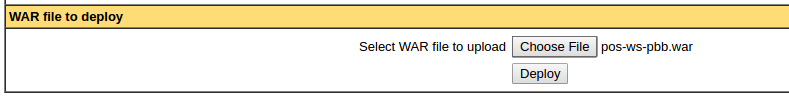
\includegraphics[width=1\textwidth]{./resources/001-deploy-war}
    \caption{\textit{Deploy File} \texttt{war}}
    \label{fig:deploy-war}
  \end{figure}
  
  \item Melakukan pengujian dengan melakukan akses ke \textit{server} menggunakan \textit{browser}, hasilnya akan terlihat seperti pada gambar \ref{fig:ws-worked} berikut :
  
  \begin{figure}[H]
    \centering
    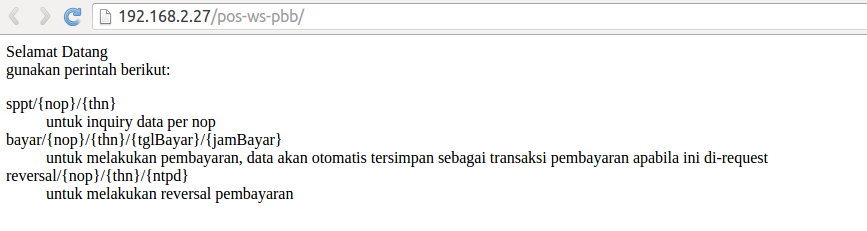
\includegraphics[width=1\textwidth]{./resources/002-ws-worked}
    \caption{Akses ke \textit{Web Service} Sudah Dapat Dilakukan}
    \label{fig:ws-worked}
  \end{figure}
  
  \item Selesai.
\end{enumerate}

\section{PROSEDUR OPERASI}

Sebagaimana terlihat pada gambar \ref{fig:ws-worked} bahwa ada 3 (tiga) layanan \textit{web service} yang diberikan yang dapat dilakukan dengan perintah melalui URL \textit{web} seperti berikut :

\begin{enumerate}[1.]
  \item \textit{Inquiry}
  \item Pencatatan Pembayaran
  \item \textit{Reversal} Pembayaran
\end{enumerate}

Dengan menggunakan \textit{web service} maka hanya ada 2 (dua) informasi dasar yang terjadi, yaitu berupa \textit{request} dan respon dalam dalam kata lain adalah \textit{input} dan \textit{output}. Penjelasan lebih rinci dari tiap layanan yang diberikan adalah sebagai berikut :

\subsection{\textit{Inquiry}}

Untuk \textit{inquiry} data tagihan, format \textit{request} yang dikirimkan adalah sebagai berikut :

\begin{lstlisting}
/sppt/{nop}/{thn}
\end{lstlisting}

Dengan keterangan sebagai berikut :

\begin{itemize}
  \item Parameter \texttt{\{nop\}} digantikan dengan Nomor Objek Pajak (NOP) untuk mengidentifikasi objek mana yang akan diambil informasinya.
  \item Parameter \texttt{\{thn\}} digantikan dengan Tahun Pajak untuk objek pajak yang akan diakses informasinya.
\end{itemize}

Hasil dari \textit{inquiry} di atas akan menghasilkan beberapa respon dari \textit{server}. Karena beberapa sebab, \textit{server} mungkin saja tidak dapat melakukan proses terhadap \textit{request} yang datang, sehingga diperlukan informasi yang cukup jelas sebagai informasi kepada \textit{client} bahwa \textit{request} yang dikirimkan berhasil atau gagal. 

Respon yang dikirimkan oleh \textit{server} akan menjadi bermacam-macam sesuai kondisinya, untuk memudahkan penjelasan, maka akan dibagi menjadi beberapa skenario berikut :

\begin{itemize}
  \item Skenario \textit{Inquiry} Yang Sukses
  \item Skenario \textit{Inquiry} Yang Gagal Karena Tahun Pajak Bukan Angka
  \item Skenario \textit{Inquiry} Yang Gagal Karena Data Tidak Ditemukan
  \item Skenario \textit{Inquiry} Yang Gagal Karena Kesalahan Server
\end{itemize}

Secara rinci akan dijelaskan sebagai berikut :

\subsubsection{Skenario \textit{Inquiry} Yang Sukses}

  Pada saat \textit{client} melakukan \textit{request inquiry} data ke \textit{server}, jika memang data tersebut ada pada basis data dan komunikasi berjalan sebagaimana mestinya, maka \textit{server} akan memberikan respon sebagai berikut :
  
  \begin{lstlisting}
{
  "code": 01,
  "message":"Data ditemukan",
  "sppt": {
    "nop":{nop},
    "thn":{thn},
    "nama":{nama wp},
    "alamatOp":{alamat op},
    "pokok":{pokok},
    "denda":{denda}
  }
}
  \end{lstlisting}
  
  Dengan keterangan sebagai berikut :
  
  \begin{itemize}
    \item \texttt{"code"}, berisi kode status respon dari \textit{server} yang menggambarkan suatu kondisi, jika kondisi \textit{inquiry} selesai di proses tanpa ada masalah, maka akan bernilai \texttt{01}.
    
    \item \texttt{"message"}, berisi pesan informasi dari kondisi respon \textit{server} yang telah terjadi, untuk menjelaskan kode status yang tertera pada bagian \texttt{"code"}.
    
    \item \texttt{"sppt"}, berisi informasi \textit{inquiry} yang di\textit{request} oleh \textit{client}.
    
    \item \texttt{\{nop\}}, nantinya akan terisi oleh Nomor Objek Pajak PBB-P2 yang di\textit{request} oleh \textit{client}.
    
    \item \texttt{\{thn\}}, nantinya akan terisi oleh tahun pajak untuk nomor objek pajak yang di\textit{request} oleh \textit{client}.
    
    \item \texttt{\{nama wp\}}, nantinya akan terisi oleh nama wajib pajak untuk nomor objek pajak dan tahun pajak yang diminta oleh \textit{client}.
    
    \item \texttt{\{alamat op\}}, nantinya akan terisi oleh alamat objek pajak untuk nomor objek pajak dan tahun pajak yang diminta oleh \textit{client}.
    
    \item \texttt{\{pokok\}}, nantinya akan terisi oleh besarnya pokok pajak terhutang.
    
    \item \texttt{\{denda\}}, nantinya akan terisi oleh besarnya denda administrasi yang harus dibayarkan oleh wajib pajak. Bila tanggal jatuh tempo belum terlewati, maka akan bernilai 0 (nol), namun apabila tanggal \textit{request} terjadi setelah tanggal jatuh tempo, maka nilainya akan muncul.
  \end{itemize}

\subsubsection{Skenario \textit{Inquiry} Yang Gagal Karena Tahun Pajak Bukan Angka}

  Bila ternyata karena kesalahan \textit{entry} data, tiba-tiba ada karakter bukan angka terselip pada parameter \texttt{tahun} pada saat \textit{request inquiry} data, maka \textit{server} akan menghasilkan respon berikut :

  \begin{lstlisting}
{
  "code":36,
  "message: "Tahun Pajak Mengandung Karakter bukan Angka",
  "sppt":null
}
  \end{lstlisting}

  Keterangan dari kode di atas adalah sebagai berikut :

  \begin{itemize}
    \item \texttt{\"code\"}, ini berisi kode pesan respon yang dihasilkan \textit{server} setelah menerima \textit{request} dari \textit{client}. Kode ini akan menyimbolkan sesuatu yang terjadi di \textit{server} untuk kemudian dikembalikan sebagai respon ke \textit{client}.
    
    \item \texttt{\"message\"}, berisi keterangan untuk menjelaskan mengenai kode yang dihasilkan pada bagian \texttt{\"code\"}. Pada bagian ini dijelaskan bahwa ternyata \textit{client} telah mengirimkan parameter tahun pajak yang mengandung karakter bukan angka. Sebagai contoh, misalkan bahwa \textit{client} ternyata mengirimkan parameter tahun pajak dengan nilai \texttt{2p16}, sehingga \textit{server} akan mengirimkan respon seperti diatas.
    
    \item \texttt{\"sppt\"}, akan berisi \texttt{null} yang boleh diartikan kosong, karena data \textit{inquiry} yang diminta oleh \textit{client} memiliki kesalahan sehingga datanya tidak dapat diproses.
  \end{itemize}

\subsubsection{Skenario \textit{Inquiry} Yang Gagal Karena Data Tidak Ditemukan}

  Pada skenario ini, \textit{client} dengan benar memberikan parameter Nomor Objek Pajak dan tahun pajak yang diinginkan tanpa ada kesalahan pengetikan, namun ternyata setelah data dicari dalam basis data dengan menggunakan parameter yang disediakan, data tersebut tidak ada dalam basis data, sehingga respon yang dihasilkan \textit{server} akan terlihat sebagai berikut :
  
  \begin{lstlisting}
{
  "code":10,
  "message":"Data Tidak Ditemukan",
  "sppt":null
}
  \end{lstlisting}
  
  \begin{itemize}
    \item \texttt{\"code\"}, bagian ini akan berisi kode pesan yang dihasilkan \textit{server} sebagai respon terhadap \textit{request} dari \textit{client}. Kode yang dihasilkan untuk skenario ini adalah \texttt{10}.
    
    \item \texttt{\"message\"}, bagian ini akan berisi deskripsi atau penjelasan dari kode yang dihasilkan pada bagian \texttt{\"code\"}. Untuk skenario ini, pesan yang dihasilkan adalah \texttt{\"Data Tidak Ditemukan\"} karena memang data yang diminta oleh \textit{client} tidak ada pada basis data.
    
    \item \texttt{\"sppt\"}, karena proses \textit{inquiry} tidak berhasil dengan data yang tidak ditemukan dalam basis data, maka isi dari parameter \texttt{\"sppt\"} ini pun akan bernilai \texttt{null} yang artinya kosong.
  \end{itemize}

\subsubsection{Skenario \textit{Inquiry} Yang Gagal Karena Kesalahan Server}

  Pada skenario kali ini, \textit{client} dengan benar mengirimkan parameter \textit{request} ke \textit{server}, namun kegagal terjadi pada saat \textit{server} aplikasi akan mengambil data pada sistem basis data. Respon yang dihasilkan oleh \textit{server} untuk kondisi seperti ini adalah sebagai berikut :
  
  \begin{lstlisting}
{
  "code":04,
  "message":"Kesalahan DB",
  "sppt":null
}
  \end{lstlisting}
  
  Penjelasan untuk kode di atas adalah sebagai berikut :
  
  \begin{itemize}
    \item \texttt{\"code\"}, bagian ini akan berisi status kode respon yang diberikan oleh \textit{server} pada \textit{client}, karena terjadi kesalahan komunikasi antara \textit{server} aplikasi dengan \textit{server} basis data, sehingga kode yang dihasilkan adalah kode \texttt{04}.
    
    \item \texttt{\"message\"}, bagian ini akan berisi penjelasan dari kode yang diberikan diatas, informasi yang diberikan yaitu \textit{\"Kesalahan DB\"}, yang dimaksud adalah adanya kesalahan yang terjadi antara \textit{server} aplikasi yang melakukan \textit{request} data ke \textit{server} basis data.
    
    \item \texttt{\"sppt\"}, tentunya parameter ini akan bernilai \texttt{null} karena tidak ada data PBB-P2 yang bisa dikirimkan ke \textit{client}.
  \end{itemize}

\subsection{Pencatatan Pembayaran}

  Untuk pencatatan pembayaran, format \textit{request} yang dapat dikirimkan oleh \textit{client} ke \textit{server} adalah sebagai berikut :
  
  \begin{lstlisting}
/bayar/{nop}/{thn}/{tglBayar}/{jamBayar}
  \end{lstlisting}
  
  Keterangan untuk format \textit{request} di atas adalah sebagai berikut :
  
  \begin{itemize}
    \item Parameter \texttt{\{nop\}}, nantinya diisikan dengan Nomor Objek Pajak yang akan dicatatkan pembayarannya.
    
    \item Parameter \texttt{\{thn\}}, nantinya diisikan dengan tahun pajak untuk nomor objek pajak yang akan dicatatkan pembayarannya.
    
    \item Parameter \texttt{\{tglBayar\}}, nantinya diisikan dengan tanggal terjadinya transaksi pembayaran.
    
    \item Parameter \texttt{\{jamBayar\}}, nantinya diisikan dengan jam terjadinya transaksi pembayaran.
  \end{itemize}
  
  Dari \textit{request} pencatatan transaksi pembayaran yang terjadi seperti di atas, hasil respon yang dikirimkan \textit{server} ke \textit{client} akan terbagai menjadi beberapa skenario berikut :
  
  \begin{itemize}
    \item Skenario Pencatatan Transaksi Pembayaran Yang Sukses.
    \item Skenario Pencatatan Transaksi Pembayaran Yang Gagal Karena Tanggal dan Jam Pembayaran Telah Melewati Tanggal dan Jam Pencatatan.
    \item Skenario Pencatatan Transaksi Pembayaran Yang Gagal Karena Tagihan Telah Terbayar Atau Bernilai Nihil.
    \item Skenario Pencatatan Transaksi Pembayaran Yang Gagal Karena Tagihan Telah Dibatalkan.
    \item Skenario Pencatatan Transaksi Pembayaran Yang Gagal Karena Terjadi Kesalahan di Sisi Server.
  \end{itemize}
  
  Secara rinci, setiap skenario akan dijelaskan pada bagian-bagian berikut :
  
  \subsubsection{Skenario Pencatatan Transaksi Pembayaran Yang Sukses}
  
  Saat \textit{client} mengirimkan \textit{request} pencatatan transaksi pembayaran yang benar dengan data tagihan pada sistem basis data ada dan belum terbayar, maka \textit{server} akan menghasilkan respon sebagai berikut :
  
  \begin{lstlisting}
{
  "code":01,
  "message":"Pembayaran Telah Tercatat",
  "byrSppt":{
    "nop":{nop},
    "thn":{thn},
    "ntpd":{ntpd},
    "mataAnggaranPokok":{mataAnggaranPokok},
    "pokok":{pokok},
    "mataAnggaranSanksi":{mataAnggaranSanksi},
    "sanksi":{sanksi},
    "namaWp":{namaWp},
    "alamatOp":{alamatOp}
  }
}
  \end{lstlisting}
  
  Penjelasan dari kode respon \textit{respon} di atas adalah sebagai berikut :
  
  \begin{itemize}
    \item Parameter \texttt{\"code\"} akan berisi kode status respon dari \textit{server}, dalam kondisi skenario ini akan bernilai \texttt{01}.
    
    \item Parameter \texttt{\"message\"} akan berisi penjelasan dari kode status pada parameter \texttt{\"code\"}. Untuk skenario ini, parameter \texttt{\"message\"} akan berisi \texttt{Pembayaran Telah Tercatat}.
    
    \item Parameter \texttt{\"byrSppt\"} yang isinya adalah informasi hasil pencatatan transaksi pembayaran pada basis data.
    
    \item Parameter \texttt{\{nop\}}, nantinya akan terisi oleh Nomor Objek Pajak untuk PBB-P2 yang dicatatkan pembayarannya.
    
    \item Parameter \texttt{\{thn\}}, nantinya akan terisi oleh tahun pajak untuk nomor pajak PBB-P2 yang dicatatkan pembayarannya.
    
    \item Parameter \texttt{\{ntpd\}}, nantinya akan terisi oleh Nomor Transaksi Pajak Daerah yang berupa kode unik untuk tiap transaksi yang terjadi.
    
    \item Parameter \texttt{\{mataAnggaranPokok\}}, nantinya akan terisi informasi kode mata anggaran penerimaan untuk pokok pajak PBB-P2.
    
    \item Parameter \texttt{\{pokok\}}, nantinya akan terisi besarnya pokok pajak PBB-P2 yang terbayar
    
    \item Parameter \texttt{\{mataAnggaranSanksi\}}, nantinya akan terisi informasi kode mata anggaran penerimaan untuk sanksi administratif berupa denda pajak.
    
    \item Parameter \texttt{\{sanksi\}}, nantinya akan terisi besarnya sanksi administratif, atau dendan pajak yang terbayar untuk PBB-P2.
    
    \item Parameter \texttt{\{namaWp\}}, nantinya akan terisi dengan nama wajib pajak untuk nomor objek pajak pada tahun pajak yang di \textit{request} oleh \textit{client}.
    
    \item Parameter \texttt{\{alamatOp\}}, nantinya akan terisi dengan alamat objek pajak.
  \end{itemize}
  
  \subsubsection{Skenario Pencatatan Transaksi Pembayaran Yang Gagal Karena Tanggal dan Jam Pembayaran Telah Melewati Tanggal dan Jam Pencatatan}
  
  Pada saat \textit{client} mengirimkan \textit{request} pencatatan transaksi pembayaran, maka \textit{client} akan mengirimkan informasi tanggal dan jam terjadinya transaksi pembayaran, namun apabila tanggal dan jam terjadinya pembayaran telah melewati tanggal dan jam pencatatan, maka kondisinya akan gagal dicatatkan dan \textit{server} akan mengirimkan respon berikut :
  
  \begin{lstlisting}
{
  "code":32,
  "message":"Tanggal atau jam pada saat dibayarkan melebihi tanggal dan jam saat ini",
  "byrSppt":null
}
  \end{lstlisting}
  
  Penjelasan untuk kode di atas adalah sebagai berikut :
  
  \begin{itemize}
    \item Parameter \texttt{\"code\"}, berisi kode status pencatatan pembayaran yang terjadi di \textit{server}, pada skenario ini akan berisi \texttt{32}.
    \item Parameter \texttt{\"message\"}, berisi pesan yang menjelaskan kode status yang berada pada parameter \texttt{\"code\"} di atas, pada skenario ini akan berisi pesan \texttt{Tanggal atau jam pada saat dibayarkan melebihi tanggal dan jam saat ini}.
    \item Parameter \texttt{\"byrSppt\"}, karena proses pencatatan transaksi pembayaran pada skenario ini tidak berhasil, maka isi dari parameter ini adalah \texttt{null}.
  \end{itemize}
  
  \subsubsection{Skenario Pencatatan Transaksi Pembayaran Yang Gagal Karena Tagihan Telah Terbayar Atau Bernilai Nihil}
  
  Pada saat \textit{client} melakukan \textit{request} pencatatan transaksi pembayaran ke \textit{server}, ternyata parameter tanggal dan jam pembayaran telah melewati tanggal dan jam pencatatan (hari dan jam saat terjadinya \textit{request} ini), maka \textit{server} akan mengirimkan pesan respon sebagai berikut :
  
  \begin{lstlisting}
{
  "code":32,
  "message":"Tanggal atau jam pada saat dibayarkan melebihi tanggal dan jam saat ini",
  "byrSppt":null
}
  \end{lstlisting}
  
  Penjelasan untuk pesan respon di atas adalah sebagai berikut :
  
  \begin{itemize}
    \item Parameter \texttt{\"code\"} adalah kode status respon yang dikirimkan oleh \textit{server} untuk menggambarkan hasil proses dari \textit{request} yang telah dikirimkan oleh \textit{client}.
    \item Parameter \texttt{\"message\"} adalah pesan penjelas yang mendeskripsikan kode yang ada pada parameter \texttt{\"code\"}. Pada skenario ini, akan muncul pesan berikut : \texttt{Tanggal atau jam pada saat dibayarkan melebihi tanggal dan jam saat ini}.
    \item Parameter \texttt{\"byrSppt\"} akan bernilai \texttt{null} karena memang \textit{request} tidak berhasil diselesaikan oleh \textit{server} karena ada kesalahan isian parameter.
  \end{itemize}
  
  \subsubsection{Skenario Pencatatan Transaksi Pembayaran Yang Gagal Karena Tagihan Telah Dibatalkan}
  
  Pada skenario ini, \textit{client} mengirimkan \textit{request} pencatatan transaksi pembayaran ke \textit{server}, yang ternyata tagihan untuk nomor objek pajak dan tahun pajak yang diminta sudah dibatalkan, sehingga tidak ada tagihan pajak terhutang. \textit{Server} kemudian akan mengirimkan respon sebagai berikut :
  
  \begin{lstlisting}
{
  "code":03,
  "message":"Tagihan SPPT Telah Dibatalkan",
  "byrSppt":null
}
  \end{lstlisting}
  
  Penjelasan untuk kode respon di atas adalah sebagai berikut :
  
  \begin{itemize}[H]
    \item Parameter \texttt{\"code\"} berisi kode status respon \textit{server} terhadap \textit{request} dari \textit{client}.
    \item Parameter \texttt{\"message\"} berisi penjelasan atas kode status yang tertera pada parameter \texttt{\"code\"}.
    \item Parameter \texttt{\"byrSppt\"} berisi \texttt{null} karena memang proses pencatatan transaksi pembayaran gagal sehingga tidak ada informasi mengenai objek pajak yang dikirimkan ke \textit{client}.
  \end{itemize}
  
  \subsubsection{Skenario Pencatatan Transaksi Pembayaran Yang Gagal Karena Terjadi Kesalahan di Sisi Server}  
  
  Pada saat \textit{client} mengirimkan \textit{request} pencatatan transaksi pembayaran, format dan isi dari tiap parameter masukkan sudah benar, hanya saja pada saat \textit{server} aplikasi akan mengambil data pada \textit{server} basis data mengalami kegagalan. Berikut respon yang dikirimkan oleh \textit{server} sebagai jawaban atau respon dari \textit{request client} :
  
  \begin{lstlisting}
{
  "code":04,
  "message":"Kesalahan Server",
  "byrSppt":null
}
  \end{lstlisting}

  Penjelasan untuk isi kode di atas adalah sebagai berikut :
  
  \begin{itemize}
    \item Parameter \texttt{\"code\"} berisi kode status respon \textit{server} terhadap \textit{request} dari \textit{client}. Pada skenario ini berisi \texttt{04}.
    \item Parameter \texttt{\"message\"} berisi penjelasan dari kode status respon yang berada pada parameter \texttt{\"code\"}, pada skenario ini berisi \texttt{\"Kesalahan Server\"}, karena memang \textit{server} gagal memproses data yang dikirimkan oleh \textit{client}.
    \item Parameter \texttt{\"byrSppt\"} berisi \texttt{null} karena memang proses pencatatan transaksi pembayaran gagal di proses.
  \end{itemize}
  
\subsection{\textit{Reversal} Pembayaran}

  \textit{Reversal} Pembayaran dilakukan apabila ada kesalahan pencatatan pembayaran yang sebelumnya terjadi. Untuk melakukan \textit{request reversal} pembayaran ini, format yang dikirimkan adalah sebagai berikut :

  \begin{lstlisting}
/reversal/{nop}/{thn}/{ntpd}
  \end{lstlisting}
  
  Penjelasan untuk format \textit{request} di atas adalah sebagai berikut :
  
  \begin{itemize}
    \item Parameter \texttt{\{nop\}} digantikan dengan nomor objek pajak yang pencatatan pembayarannya akan dilakukan \textit{reversal}.
    \item Parameter \texttt{\{thn\}} digantikan dengan tahun pajak untuk nomor objek pajak yang pencatatan pembayarannya akan dilakukan \textit{reversal}.
    \item Parameter \texttt{\{ntpd\}} digantikan dengan nomor transaksi pajak daerah yang didapatkan pada saat melakukan \textit{request} pencatatan transaksi pembayaran.
  \end{itemize}
  
  Respon dari \textit{server} untuk \textit{request} di atas akan terbagi menjadi beberapa skenario sebagai berikut :
  
  \begin{itemize}
    \item Skenario \textit{Reversal} Pembayaran Yang Sukses
    \item Skenario \textit{Reversal} Pembayaran Yang Gagal Karena Data Yang Diminta Tidak Ada.
    \item Skenario \textit{Reversal} Pembayaran Yang Gagal Karena Ada Data Pembayaran Yang Tercatat Ganda.
    \item Skenario \textit{Reversal} Pembayaran Yang Gagal Karena Kesalahan \textit{Server}
  \end{itemize}
  
  Secara rinci, tiap skenario di atas akan dijelaskan pada bagian-bagian berikut :
  
  \subsubsection{Skenario \textit{Reversal} Pembayaran Yang Sukses}
  
  Pada skenario ini, \textit{client} mengirimkan \textit{request} atau permintaan \textit{reversal} pembayaran karena terjadi kesalahan pencatatan pembayaran sebelumnya. \textit{Request} yang dikirimkan \textit{client} ke \textit{server} adalah seperti dijelaskan diatas, kemudian \textit{server} memberikan respon yang menyatakan bahwa proses \textit{reversal} telah selesai dilaksanakan dan berhasil, berikut kode respon yang dikirim oleh \textit{server} ke \textit{client} :
  
  \begin{lstlisting}
{
  "code":01,
  "message":"Proses Reversal Berhasil",
  "revPembayaran":{
    "nop":{nop},
    "thn":{thn},
    "ntpd":{ntpd}
  }
}
  \end{lstlisting}
  
  Penjelasan untuk kode respon di atas adalah sebagai berikut :
  
  \begin{itemize}
    \item Parameter \texttt{code}, berisi kode status respon yang dikirimkan dari \textit{server} ke \textit{client} yang menandakan berhasil atau tidaknya proses \textit{reversal} dilakukan di sisi \textit{server}.
    \item Parameter \texttt{message}, berisi penjelasan dari kode status respon pada parameter \texttt{code}. Pada skenario ini isinya berupa pesan \texttt{Proses Reversal Berhasil}.
    \item Parameter \texttt{revPembayaran}, berisi informasi transaksi mana yang berhasil dilakukan \textit{reversal}.
    \item Parameter \texttt{\{nop\}}, berisi nomor objek pajak yang akan dilakukan \textit{reversal} pembayaran.
    \item Parameter \texttt{\{thn\}}, berisi tahun pajak untuk nomor objek pajak yang akan dilakukan \textit{reversal} pembayaran.
    \item Parameter \texttt{\{ntpd\}}, berisi nomor transaksi pajak daerah untuk objek pajak dan tahun pajak yang akan dilakukan \textit{reversal} pembayaran.
  \end{itemize}
  
  \subsubsection{Skenario \textit{Reversal} Pembayaran Yang Gagal Karena Data Yang Diminta Tidak Ada}
  
  Pada skenario ini, \textit{client} mengirimkan permintaan \textit{reversal} pembayaran ke \textit{server}, namun setelah \textit{server} aplikasi melakukan pemeriksaan data pada \textit{server} sistem basis data, data yang diminta untuk dilakukan \textit{reversal} pembayaran tidak ada, sehingga \textit{server} akan memberikan respon berikut :
  
  \begin{lstlisting}
{
  "code":10,
  "message":"Data Yang Diminta Tidak Ada",
  "revPembayaran":null
}
  \end{lstlisting}
  
  Penjelasan untuk kode respon di atas adalah sebagai berikut :
  
  \begin{itemize}
    \item Parameter \texttt{code}, berisi kode status respon yang dikirimkan \textit{server} ke \textit{client} yang menandakan berhasil atau tidaknya proses \textit{reversal} dilakukan di sisi \textit{server}.
    \item Parameter \texttt{message}, berisi penjelasan atas kode yang muncul pada parameter \texttt{code}, untuk skenario ini berisi pesan \texttt{Data Yang Diminta Tidak Ada}.
    \item Parameter \texttt{revPembayaran}, berisi informasi objek pajak, tahun pajak, dan nomor transaksi \textit{reversal} pembayaran yang telah dilakukan, karena pada skenario ini proses \textit{reversal} gagal dilakukan, maka bernilai \texttt{null}.
  \end{itemize}
  
  \subsubsection{Skenario \textit{Reversal} Pembayaran Yang Gagal Karena Ada Data Pembayaran Yang Tercatat Ganda}
  
  Pada skenario ini, \textit{client} mengirimkan permintaan \textit{reversal} pembayaran ke \textit{server}, namun \textit{server} gagal melakukan proses \textit{reversal} karena pada saat pencatatan transaksi pembayaran terjadi pencatatan ganda dengan nomor objek pajak, tahun pajak, dan nomor transaksi pajak daerah yang sama. \textit{Server} kemudian akan mengirimkan pesan respon sebagai berikut :
  
  \begin{lstlisting}
{
  "code":04,
  "message":"Data tersebut Ganda",
  "revPembayaran":null
}
  \end{lstlisting}
  
  Penjelasan untuk kode respon di atas adalah sebagai berikut :
  
  \begin{itemize}
    \item Parameter \texttt{code}, berisi kode status respon dari \textit{server} yang menandakan status berhasil atau tidaknya proses \textit{reversal} pembayaran dilakukan.
    \item Parameter \texttt{message}, berisi pesan penjelas atas kode yang terisi pada parameter \texttt{code}, yang pada skenario ini berisi \texttt{Data tersebut Ganda}.
    \item Parameter \texttt{revPembayaran}, yang isinya bernilai \texttt{null} karena memang proses \textit{reversal} pembayaran gagal dilakukan.
  \end{itemize}
  
  \subsubsection{Skenario \textit{Reversal} Pembayaran Yang Gagal Karena Kesalahan \textit{Server}}
  
  Pada skenario ini, \textit{client} akan mengirimkan permintaan \textit{reversal} pembayaran ke \textit{server}, namun saat \textit{server} aplikasi melakukan komunikasi dengan \textit{server} sistem basis data, terjadi gangguan sehingga proses \textit{reversal} pembayaran tidak dapat dilanjutkan. Pada kondisi ini, \textit{server} akan mengirimkan respon sebagai berikut :
  
  \begin{lstlisting}
{
  "code":04,
  "message":"Kesalahan Server",
  "revPembayaran":null
}
  \end{lstlisting}
  
  Penjelasan untuk kode respon di atas adalah sebagai berikut :
  
  \begin{itemize}
    \item Parameter \texttt{code}, berisi kode status respon dari \textit{server} yang menandakan status berhasil atau tidaknya proses \textit{reversal} pembayaran dilakukan.
    \item Parameter \texttt{message}, berisi pesan penjelas atas kode yang terisi pada parameter \texttt{code}, yang pada skenario ini berisi \texttt{Kesalahan Server}.
    \item Parameter \texttt{revPembayaran}, yang isinya bernilai \texttt{null} karena memang proses \textit{reversal} pembayaran gagal dilakukan.
  \end{itemize}

\section{REFERENSI KODE}

Dari tiap respon yang dikirimkan oleh \textit{server} ke \textit{client} sebagai jawaban atas tiap \textit{request}, maka \textit{server} akan mengirimkan kode pada parameter \texttt{code}. Isi dari parameter \texttt{code} ini dapat dilihat pada daftar berikut beserta penjelasannya :

\begin{itemize}
  \item \texttt{01}, artinya permintaan proses yang dikirimkan oleh \textit{client} ke \textit{server} berhasil dilakukan dengan sempurna.
  \item \texttt{10}, artinya data nomor objek pajak untuk tahun pajak yang diinginkan oleh \textit{client} tidak ada pada sistem basis data.
  \item \texttt{13}, artinya nomor objek pajak untuk tahun pajak yang diminta oleh \textit{client} sudah pernah dilakukan pembayaran sebelumnya.
  \item \texttt{03}, artinya nomor objek pajak untuk tahun pajak yang diminta oleh \textit{client} bernilai nihil, tidak ada nilai pajak terhutang.
  \item \texttt{04}, artinya \textit{server} aplikasi tidak dapat berkomunikasi dengan \textit{server} sistem basis data.
  \item \texttt{05}, artinya \textit{server} tidak berhasil melakukan pembentukan nomor transaksi pajak daerah.
  \item \texttt{31}, artinya parameter jumlah pembayaran yang dikirimkan oleh \textit{client} mengandung karakter bukang angka.
  \item \texttt{32}, artinya parameter tanggal dan jam pembayaran telah melewati tanggal dan jam pencatatan
  \item \texttt{33}, artinya parameter tanggal dan jam terjadinya permintaan \textit{reversal} sudah melebihi 24 (dua puluh empat) jam.
  \item \texttt{34}, artinya kode \textit{request} yang dikirimkan oleh \textit{client} tidak benar dan tidak dapat diproses.
  \item \texttt{35}, artinya masa pajak yang dikirimkan oleh \textit{client} sebagai sebuah \textit{request} memiliki karaketer bukan angka.
  \item \texttt{36}, artinya parameter tahun pajak yang dikirim oleh \textit{client} mengandung karakter bukang angka.
\end{itemize}

\end{document}